\documentclass{../../test-template}

\begin{document}

\begin{center}
    \textbf{\Huge{Homework №1.} \\ \large Шифр Цезаря. Шифр Віженера.}
\end{center}

\section*{Теоретична зноска.}

\begin{tcolorbox}[breakable, colback=gray!10!white,fonttitle=\bfseries,colframe=blue!80!black,title=Афінний шифр]
Нехай задано ключову пару на $\mathbb{Z}_m$ -- $(a,b)$, де $a\in \mathbb{Z}^*_m,b\in \mathbb{Z}_m$, $(a,m)=1$. Тоді шифрування відбувається за правилом:
\begin{equation*}
    y_i=(a\cdot x_i +b)\texttt{ mod }m.
\end{equation*}
Щоб розшифрувати повідомлення, необхідно обчислити $a^{-1}\texttt{ mod } m$ та виконати перетворення
\begin{equation*}
    x_i=a^{-1}(y_i-b)\texttt{ mod }m.
\end{equation*}

\end{tcolorbox}

\begin{tcolorbox}[breakable, colback=gray!10!white,fonttitle=\bfseries,colframe=blue!80!black,title=Шифр Віженера]
Нехай задано послідовність на $\mathbb{Z}_m$ -- ключ $K=k_1k_2...k_r\in(\mathbb{Z}_m)^r$. Тоді шифрування відкритого тексту $M=m_1m_2...m_k$ відбуватиметься за правилом:
\begin{equation*}
    c_i=m_i+k_{i\texttt{ mod }r}\texttt{ mod }m.
\end{equation*}
Щоб розшифрувати повідомлення, необхідно виконати зворотне перетворення:
\vspace{-3mm}
\begin{equation*}
    m_i=c_i-k_{i\texttt{ mod }r}\texttt{ mod }m.
\end{equation*}

\end{tcolorbox}

\begin{tcolorbox}[breakable, colback=gray!10!white,fonttitle=\bfseries,colframe=purple!80!black,title=Обчислення оберненого елемента за модулем]
Нехай $(a,b)=1$. Тоді, елемент $a^{-1} \texttt{ mod }b$ називають \textbf{оберненим за модулем}, якщо
\begin{equation*}
    a\cdot a^{-1}\equiv1\texttt{ mod }b.
\end{equation*}
З властивостей НСД можна отримати, що 
\begin{equation*}
    (a,b)=1\Rightarrow \exists u,v\in \mathbb{Z}: 1=u\cdot a+v\cdot b
\end{equation*}
Тоді, можна отримати:

\vspace{-9mm}
\begin{gather*}
    1=ua\texttt{ mod }b; \\
    a^{-1}=u\texttt{ mod }b.
\end{gather*}
Табличним способом:

\centering
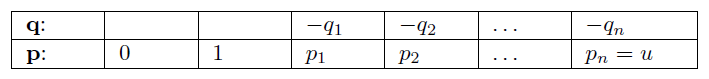
\includegraphics[width=0.55\linewidth]{templates/1-number-theory/table_meth.png}

\vspace{-5mm}
\begin{gather*}
    a=q_1\cdot b+r_2 \\
    b=q_2\cdot r_2+r_3 \\
    ...
    \\
     r_{k-1}=q_k\cdot r_k+r_{k+1}, \quad r_{k+1}=0, \quad   \\ 
     r_k=(r_0,r_1)
\end{gather*}
\end{tcolorbox}

\newpage
\section*{Задачі}
\subsection{Шифр Цезаря. Афінний шифр}
\begin{figure}
    \centering
    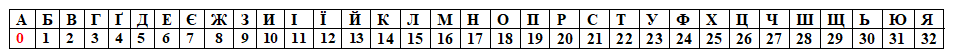
\includegraphics[width=0.95\linewidth]{1-crypto-practice/images/c3.png}
    \label{fig:placeholder}
\end{figure}
\begin{tcolorbox}[lowerbox=invisible,colback=white]
    \begin{minipage}{0.1\textwidth}
        \raggedright
        \vspace*{\fill}
            \textbf{Q1}
        \vspace*{\fill}
        \end{minipage}
        \begin{minipage}{0.75\textwidth}
            Знайти розв'язок
            \begin{enumerate}[(A)]
                \item $17^{-1}\texttt{ mod }123$.
                \item $19^{-1}\texttt{ mod }323$.
                \item $16x\equiv85 \texttt{ mod }113$
                \item $328x\equiv20 \texttt{ mod }96$
            \end{enumerate}
        \end{minipage}
\end{tcolorbox}

\begin{tcolorbox}[lowerbox=invisible,colback=white]
    \begin{minipage}{0.1\textwidth}
        \raggedright
        \vspace*{\fill}
            \textbf{Q2}
        \vspace*{\fill}
        \end{minipage}
        \begin{minipage}{0.75\textwidth}
            Нехай задано афінний шифр із ключовою парою $(a,b)=(7,2)$. Зашифруйте повідомлення "КОРОЛЬ".
        \end{minipage}
\end{tcolorbox}

\begin{tcolorbox}[lowerbox=invisible,colback=white]
    \begin{minipage}{0.1\textwidth}
        \raggedright
        \vspace*{\fill}
            \textbf{Q3}
        \vspace*{\fill}
        \end{minipage}
        \begin{minipage}{0.75\textwidth}
             Нехай задано афінний шифр із ключовою парою $(a,b)=(4,4)$. Розшифруйте повідомлення "ЕҐОЬЦИ".
        \end{minipage}
\end{tcolorbox}

\begin{tcolorbox}[lowerbox=invisible,colback=white]
    \begin{minipage}{0.1\textwidth}
        \raggedright
        \vspace*{\fill}
            \textbf{Q4}
        \vspace*{\fill}
        \end{minipage}
        \begin{minipage}{0.75\textwidth}
            Нехай задано шифр Цезаря з автоключем, де шифрування відбувається за правилом:
            \begin{gather*}
            c_0=(m_0+k)\textsf{ mod }n,\\
        c_i=(m_{i-1}+m_i)\textsf{ mod } n, \forall i\geq1.
            \end{gather*}
            Побудуйте атаку на даний шифр використовуючи підхід частотного криптоаналізу.
        \end{minipage}
\end{tcolorbox}

\begin{tcolorbox}[lowerbox=invisible,colback=white]
    \begin{minipage}{0.1\textwidth}
        \raggedright
        \vspace*{\fill}
            \textbf{Q5}
        \vspace*{\fill}
        \end{minipage}
        \begin{minipage}{0.75\textwidth}
            Нехай $n$ -- довільне число. Скільки нерухомих точок мати афінний шифр? Опишіть усі випадки
        \end{minipage}
\end{tcolorbox}


\subsection{Шифр Віженера}

\begin{tcolorbox}[lowerbox=invisible,colback=white]
    \begin{minipage}{0.1\textwidth}
        \raggedright
        \vspace*{\fill}
            \textbf{Q6}
        \vspace*{\fill}
        \end{minipage}
        \begin{minipage}{0.75\textwidth}
            Зашифруйте повідомлення <<\texttt{ЯСТАНУКОРОЛЕММАГIВ}>> шифром Віженера з ключем <<\texttt{КОНЮШИНА}>>
        \end{minipage}
\end{tcolorbox}

\begin{tcolorbox}[lowerbox=invisible,colback=white]
    \begin{minipage}{0.1\textwidth}
        \raggedright
        \vspace*{\fill}
            \textbf{Q7}
        \vspace*{\fill}
        \end{minipage}
        \begin{minipage}{0.75\textwidth}
Зашифруйте теж саме повідомлення, що і в задачі \textbf{Q6} та тим самим ключем, але використовуючи шифр Віженера із автоключем.
        \end{minipage}
\end{tcolorbox}
\end{document}